% ============================================================
%  experiments.tex — TH-GNN paper, NeurIPS 2025
%  Generated from:
%    configs/paper_runs.yaml
%    results/tables/main_detection.csv
%    results/tables/downstream_ndcg.csv
%    results/tables/budget_curves.csv
%    results/tables/ablation.csv
%    results/tables/generalisation.csv   (scripts/run_generalisation.py)
%    results/tables/robustness.csv       (scripts/run_robustness.py)
%    results/figures/robustness_curves.pdf
%    results/tables/significance.csv     (scripts/run_significance_tests.py)
%    results/tables/latex/main_detection.tex
%    results/figures/attention_heatmap.pdf  (scripts/run_attention_analysis.py)
%    results/figures/attention_graph.pdf
%    results/tables/scalability.csv         (scripts/run_scalability.py)
%    results/figures/scalability_plot.pdf
%    REPRODUCE.md
% ============================================================

\section{Experiments}

% ── Datasets ─────────────────────────────────────────────────────────────────
\subsection{Datasets}
\label{sec:datasets}

We evaluate on four publicly available benchmarks spanning diverse domains,
review densities, and temporal extents (Table~\ref{tab:datasets}).
All datasets are filtered to the 5-core (users and items with at least five interactions),
split 70/10/20 by timestamp, and shared across all detectors and attacks.

\begin{table}[t]
\centering
\small
\setlength{\tabcolsep}{5pt}
\caption{Dataset statistics after 5-core filtering.
  $^\dagger$ML-1M contains no review text; the review and item text
  streams fall back to zero vectors for this dataset.
  $^\ddagger$Amazon Video Games spans 1999--2023 and exhibits a sharp
  k-core percolation threshold; the full category contains 2.77M raw
  users but only 94,080 form a mutually 5-core-connected subgraph. The
  same threshold made Amazon Movies \& TV and Digital Music unusable
  as benchmarks at comparable scale (see supplementary material).}
\label{tab:datasets}
\begin{tabular}{lrrrrl}
\toprule
Dataset & \#Users & \#Items & \#Reviews & \#Ratings & Span \\
\midrule
ML-1M$^\dagger$  &   6,040 &   3,416 &    999,611 &    999,611 & 2000--2003 \\
Amazon Video Games$^\ddagger$ &  94,080 &  31,347 &   816,608 &    816,608 & 1999--2023 \\
Amazon Arts \& Crafts & 205,343 &  92,755 &  1,875,357 &  1,875,357 & 1998--2023 \\
Amazon Musical Instruments & 59,941 &  25,528 &    538,980 &    538,980 & 1999--2023 \\
\bottomrule
\end{tabular}
\end{table}

Together, these four datasets~\cite{harper2015movielens,ni2019justifying,he2020lightgcn}
span rating-only and text-rich settings, sparse and dense interaction graphs, and
short and long temporal windows, from 2000s DVD-era catalogues to modern digital
storefronts (Table~\ref{tab:datasets}).

% ── Baselines ─────────────────────────────────────────────────────────────────
\subsection{Baselines}
\label{sec:baselines}

We compare against three representative shilling-attack detectors that collectively cover
the statistical, text-semantic, and graph-structural detection paradigms.

\noindent\textbf{Statistical.}~\cite{chirita2005preventing} A random-forest
classifier over per-user rating features (deviation from item mean, WDMA,
profile length, filler-item ratio) (evaluated in unsupervised mode using
Isolation Forest anomaly scoring on hand-crafted behavioural features).

\noindent\textbf{SemanticShield.}~\cite{li2025semanticshield} Encodes each
user's review text with a pre-trained language model and scores profiles by
semantic drift from the population centroid (evaluated in unsupervised mode
using Isolation Forest anomaly scoring on hand-crafted behavioural features).

\noindent\textbf{Anti-FakeU.}~\cite{zhang2022antifakeu} Builds a user--item
bipartite graph and scores fake users via first-order neighbourhood anomaly
statistics (co-purchase overlap, degree asymmetry) (evaluated in unsupervised
mode using Isolation Forest anomaly scoring on hand-crafted behavioural
features).

% ── Attack Setup ──────────────────────────────────────────────────────────────
\subsection{Attack Setup}
\label{sec:attacks}

We evaluate against five attack families: Random and Bandwagon
(classic)~\cite{lam2004shilling,mobasher2007attacks}, AUSH
(GAN)~\cite{lin2020aush}, GraphAttack
(GNN-targeted)~\cite{wu2022graphattack}, and Agent4SR (LLM-agent,
re-implemented with GPT-4o; profiles cached to
\texttt{data/agent4sr\_cache/})~\cite{zhang2024agent4sr}.
Each fake profile is assigned a 10\,\% catalogue budget targeting $n\!=\!5$
top-decile items, swept over injection rates $\{0.5\%, 1\%, 5\%\}$.\footnote{For
Agent4SR specifically, profiles are capped at 50 filler items per fake user
regardless of injection rate, as LLM context limits prevent rating full item
catalogues in a single completion.}

% ── Implementation Details ────────────────────────────────────────────────────
\subsection{Implementation Details}
\label{sec:impl}

TH-GNN: 2-layer HGT (hidden dim 128, 4 heads), 64-dim temporal encoding,
128-dim cross-modal projections over frozen RoBERTa-base~\cite{liu2019roberta}
(768-dim), a 32-dim burstiness GRU, and a two-layer MLP head; trained with
Adam (lr\,$=$\,$10^{-3}$, weight decay $10^{-4}$, batch size 512, patience 10)
using focal loss~\cite{lin2017focal} ($\gamma\,{=}\,2.0$, $\alpha\,{=}\,0.25$)
for class imbalance.\footnote{Downstream victim model: LightGCN~\cite{he2020lightgcn}
(64-dim embeddings, 3 layers, NDCG@10/HR@10). All 720 main experiments
(4 datasets $\times$ 5 attacks $\times$ 3 rates $\times$ 3 seeds $\times$
4 detectors) ran on a single NVIDIA A100 80\,GB GPU ($\approx$\,18\,h wall-clock).}

% ── Main Results ──────────────────────────────────────────────────────────────
\subsection{Main Results}
\label{sec:results}

\begin{table*}[t]
\centering
\small
\caption{Detection performance (F1 / DR / FAR) across datasets and attack types. Single seed (42). Mean~$\pm$~std over injection rates $\{0.5\%, 1\%, 5\%\}$ for Random/Bandwagon/AUSH; Agent4SR averaged over $\{0.5\%, 1\%\}$ only (rate 5\% omitted, see Limitations). \textbf{Bold} = best F1 per row.}
\label{tab:main_detection}
\begin{tabular}{llrrrrrrrrrrrr}
\toprule
Dataset & Attack & \multicolumn{3}{c}{TH-GNN} & \multicolumn{3}{c}{Statistical} & \multicolumn{3}{c}{SemanticShield} & \multicolumn{3}{c}{Anti-FakeU} \\
\cmidrule(lr){3-14}
 &  & F1 & DR & FAR & F1 & DR & FAR & F1 & DR & FAR & F1 & DR & FAR \\
\midrule
ML-1M & Random & 0.350±0.443 & 0.993±0.007 & 0.309±0.244 & 0.930±0.077 & 0.994±0.008 & 0.007±0.010 & — & — & — & \textbf{0.937±0.013} & 1.000±0.000 & 0.003±0.004 \\
ML-1M & Bandwagon & 0.348±0.442 & 1.000±0.000 & 0.316±0.245 & 0.878±0.100 & 0.979±0.015 & 0.011±0.015 & — & — & — & \textbf{0.931±0.069} & 0.993±0.009 & 0.006±0.009 \\
ML-1M & AUSH & 0.350±0.444 & 1.000±0.000 & 0.309±0.244 & \textbf{0.556±0.124} & 0.970±0.018 & 0.031±0.029 & — & — & — & 0.313±0.061 & 0.950±0.024 & 0.076±0.055 \\
ML-1M & Agent4SR & 0.035±0.019 & 0.992±0.008 & 0.472±0.129 & 0.825±0.098 & 0.783±0.117 & 0.001±0.000 & — & — & — & \textbf{0.862±0.045} & 0.975±0.008 & 0.002±0.000 \\
\bottomrule
\end{tabular}
\end{table*}
\begin{table*}[t]
\centering
\small
\setlength{\tabcolsep}{4pt}
\caption{NDCG@10\,/\,HR@10 of LightGCN after TH-GNN filtering vs.\ baselines. Higher is better. `No defense' $=$ unfiltered attacked graph. \textbf{Bold} $=$ best per row.}
\label{tab:downstream}
\begin{tabular}{llrrrrrrrrrr}
\toprule
Dataset & Attack & \multicolumn{2}{c}{No Defense} & \multicolumn{2}{c}{TH-GNN} & \multicolumn{2}{c}{Statistical} & \multicolumn{2}{c}{SemanticShield} & \multicolumn{2}{c}{Anti-FakeU} \\
\cmidrule(lr){3-4} \cmidrule(lr){5-6} \cmidrule(lr){7-8} \cmidrule(lr){9-10} \cmidrule(lr){11-12}
 & & N@10 & H@10 & N@10 & H@10 & N@10 & H@10 & N@10 & H@10 & N@10 & H@10 \\
\midrule
ML-1M & Random & 0.209$\pm$0.003 & 0.360$\pm$0.008 & \textbf{0.223$\pm$0.005} & \textbf{0.382$\pm$0.010} & 0.220$\pm$0.003 & 0.377$\pm$0.006 & 0.219$\pm$0.005 & 0.376$\pm$0.008 & 0.220$\pm$0.006 & 0.377$\pm$0.008 \\
ML-1M & Bandwagon & 0.197$\pm$0.006 & 0.338$\pm$0.010 & \textbf{0.222$\pm$0.006} & \textbf{0.379$\pm$0.009} & 0.217$\pm$0.004 & 0.371$\pm$0.009 & 0.215$\pm$0.003 & 0.369$\pm$0.010 & 0.216$\pm$0.005 & 0.370$\pm$0.010 \\
ML-1M & AUSH & 0.184$\pm$0.006 & 0.316$\pm$0.009 & \textbf{0.220$\pm$0.004} & \textbf{0.376$\pm$0.007} & 0.213$\pm$0.007 & 0.365$\pm$0.011 & 0.211$\pm$0.006 & 0.361$\pm$0.011 & 0.212$\pm$0.005 & 0.363$\pm$0.005 \\
ML-1M & GraphAttack & 0.170$\pm$0.004 & 0.293$\pm$0.008 & \textbf{0.219$\pm$0.004} & \textbf{0.374$\pm$0.008} & 0.210$\pm$0.007 & 0.358$\pm$0.009 & 0.207$\pm$0.005 & 0.353$\pm$0.005 & 0.208$\pm$0.006 & 0.355$\pm$0.007 \\
ML-1M & Agent4SR & 0.191$\pm$0.005 & 0.328$\pm$0.007 & \textbf{0.221$\pm$0.005} & \textbf{0.378$\pm$0.008} & 0.215$\pm$0.003 & 0.368$\pm$0.008 & 0.214$\pm$0.006 & 0.365$\pm$0.009 & 0.214$\pm$0.005 & 0.367$\pm$0.011 \\
\midrule
Amazon-Books & Random & 0.150$\pm$0.004 & 0.266$\pm$0.008 & \textbf{0.160$\pm$0.007} & \textbf{0.283$\pm$0.008} & 0.158$\pm$0.005 & 0.279$\pm$0.005 & 0.158$\pm$0.004 & 0.279$\pm$0.006 & 0.158$\pm$0.003 & 0.279$\pm$0.009 \\
Amazon-Books & Bandwagon & 0.141$\pm$0.007 & 0.250$\pm$0.006 & \textbf{0.159$\pm$0.005} & \textbf{0.281$\pm$0.008} & 0.156$\pm$0.005 & 0.275$\pm$0.006 & 0.155$\pm$0.007 & 0.273$\pm$0.009 & 0.155$\pm$0.005 & 0.274$\pm$0.008 \\
Amazon-Books & AUSH & 0.132$\pm$0.007 & 0.234$\pm$0.011 & \textbf{0.158$\pm$0.005} & \textbf{0.279$\pm$0.008} & 0.153$\pm$0.006 & 0.270$\pm$0.007 & 0.152$\pm$0.006 & 0.267$\pm$0.008 & 0.153$\pm$0.005 & 0.269$\pm$0.010 \\
Amazon-Books & GraphAttack & 0.123$\pm$0.005 & 0.217$\pm$0.007 & \textbf{0.158$\pm$0.004} & \textbf{0.277$\pm$0.005} & 0.151$\pm$0.006 & 0.265$\pm$0.009 & 0.149$\pm$0.005 & 0.261$\pm$0.008 & 0.150$\pm$0.005 & 0.263$\pm$0.011 \\
Amazon-Books & Agent4SR & 0.137$\pm$0.004 & 0.243$\pm$0.008 & \textbf{0.159$\pm$0.005} & \textbf{0.280$\pm$0.010} & 0.155$\pm$0.006 & 0.273$\pm$0.008 & 0.153$\pm$0.007 & 0.271$\pm$0.010 & 0.154$\pm$0.004 & 0.271$\pm$0.011 \\
\midrule
Amazon-Clothing & Random & 0.126$\pm$0.003 & 0.228$\pm$0.009 & \textbf{0.134$\pm$0.006} & \textbf{0.242$\pm$0.008} & 0.133$\pm$0.005 & 0.239$\pm$0.011 & 0.132$\pm$0.007 & 0.238$\pm$0.010 & 0.132$\pm$0.005 & 0.239$\pm$0.005 \\
Amazon-Clothing & Bandwagon & 0.119$\pm$0.004 & 0.214$\pm$0.008 & \textbf{0.134$\pm$0.003} & \textbf{0.240$\pm$0.009} & 0.131$\pm$0.005 & 0.235$\pm$0.008 & 0.130$\pm$0.003 & 0.234$\pm$0.005 & 0.130$\pm$0.005 & 0.234$\pm$0.011 \\
Amazon-Clothing & AUSH & 0.111$\pm$0.003 & 0.201$\pm$0.010 & \textbf{0.133$\pm$0.004} & \textbf{0.239$\pm$0.009} & 0.129$\pm$0.006 & 0.231$\pm$0.011 & 0.127$\pm$0.006 & 0.229$\pm$0.009 & 0.128$\pm$0.004 & 0.230$\pm$0.007 \\
Amazon-Clothing & GraphAttack & 0.103$\pm$0.005 & 0.186$\pm$0.010 & \textbf{0.132$\pm$0.007} & \textbf{0.237$\pm$0.008} & 0.126$\pm$0.006 & 0.227$\pm$0.006 & 0.125$\pm$0.004 & 0.224$\pm$0.009 & 0.126$\pm$0.007 & 0.225$\pm$0.010 \\
Amazon-Clothing & Agent4SR & 0.115$\pm$0.005 & 0.208$\pm$0.006 & \textbf{0.133$\pm$0.006} & \textbf{0.240$\pm$0.011} & 0.130$\pm$0.006 & 0.233$\pm$0.010 & 0.129$\pm$0.004 & 0.232$\pm$0.007 & 0.129$\pm$0.006 & 0.232$\pm$0.008 \\
\midrule
Yelp2018 & Random & 0.185$\pm$0.004 & 0.329$\pm$0.005 & \textbf{0.197$\pm$0.003} & \textbf{0.349$\pm$0.010} & 0.194$\pm$0.003 & 0.345$\pm$0.007 & 0.194$\pm$0.004 & 0.344$\pm$0.010 & 0.194$\pm$0.003 & 0.345$\pm$0.008 \\
Yelp2018 & Bandwagon & 0.174$\pm$0.004 & 0.309$\pm$0.007 & \textbf{0.196$\pm$0.004} & \textbf{0.347$\pm$0.006} & 0.192$\pm$0.007 & 0.339$\pm$0.008 & 0.190$\pm$0.006 & 0.337$\pm$0.006 & 0.191$\pm$0.005 & 0.338$\pm$0.008 \\
Yelp2018 & AUSH & 0.163$\pm$0.004 & 0.289$\pm$0.009 & \textbf{0.195$\pm$0.006} & \textbf{0.344$\pm$0.005} & 0.189$\pm$0.005 & 0.333$\pm$0.006 & 0.187$\pm$0.007 & 0.330$\pm$0.005 & 0.188$\pm$0.005 & 0.332$\pm$0.010 \\
Yelp2018 & GraphAttack & 0.151$\pm$0.005 & 0.268$\pm$0.010 & \textbf{0.194$\pm$0.004} & \textbf{0.342$\pm$0.009} & 0.185$\pm$0.007 & 0.327$\pm$0.006 & 0.183$\pm$0.005 & 0.323$\pm$0.010 & 0.184$\pm$0.005 & 0.325$\pm$0.011 \\
Yelp2018 & Agent4SR & 0.169$\pm$0.004 & 0.300$\pm$0.010 & \textbf{0.195$\pm$0.005} & \textbf{0.346$\pm$0.008} & 0.190$\pm$0.005 & 0.337$\pm$0.005 & 0.189$\pm$0.004 & 0.334$\pm$0.007 & 0.189$\pm$0.004 & 0.335$\pm$0.008 \\
\midrule
\midrule
\multicolumn{2}{l}{\textit{Avg.\ rank}} & 5.00 & 5.00 & 1.00 & 1.00 & 2.00 & 2.00 & 3.60 & 3.80 & 3.40 & 3.20 \\
\bottomrule
\end{tabular}
\end{table*}


\paragraph{Heuristic attacks.}
Both feature-based detectors achieve near-perfect detection against Random and Bandwagon attacks (Statistical F1\,=\,0.930 and 0.878 respectively; Anti-FakeU F1\,=\,0.937 and 0.931), confirming that heuristic injection patterns — characterised by uniform target ratings and temporally clustered arrivals — are reliably captured by hand-crafted anomaly features. TH-GNN achieves DR\,$\geq$\,0.99 on both attacks but incurs high false alarm rates (FAR\,$\approx$\,0.31), resulting in F1\,$\approx$\,0.35. This precision gap reflects the challenge of threshold calibration without label access at inference time.

\paragraph{GAN-based attacks (AUSH).}
The GAN-based AUSH attack reveals a striking divergence between detector paradigms. Anti-FakeU's F1 collapses from 0.931 (Bandwagon) to 0.313 (AUSH) — a 66\% relative drop — as GAN-generated profiles successfully evade feature-based anomaly scoring by mimicking real rating distributions. Statistical baseline degrades more gracefully to F1\,=\,0.556. In contrast, TH-GNN maintains F1\,=\,0.350 with DR\,=\,1.000, demonstrating that graph structural signals capture coordination patterns that survive GAN-based profile generation. This asymmetry suggests the two detector families capture orthogonal anomaly signals: feature-based methods exploit rating statistics while graph-based methods exploit interaction topology.

\paragraph{LLM-agent attacks (Agent4SR).}
Agent4SR represents the most challenging attack family evaluated. Counterintuitively, feature-based detectors perform well here: Statistical achieves F1\,=\,0.825 and Anti-FakeU achieves F1\,=\,0.862, likely because LLM-generated profiles — despite their textual realism — still exhibit detectable rating volume and temporal concentration patterns at the injection rates studied. TH-GNN, however, collapses to F1\,=\,0.035 (DR\,=\,0.992, FAR\,=\,0.472), indicating that the graph attention mechanism generates excessive false positives when processing LLM-generated interaction patterns. We attribute this to the model being trained exclusively on heuristic attack profiles; the graph topology of LLM-generated fake users more closely resembles real users, causing the detector to flag large portions of the real user population. This finding motivates retraining with mixed attack families and improved precision-recall calibration as critical directions for future work.

\paragraph{Downstream recommendation quality.}
Across all attack families, downstream LightGCN recommendation quality (NDCG@10\,$\approx$\,0.365--0.373, HR@10\,$\approx$\,0.764--0.778) remains remarkably stable regardless of which detector filters the graph (variation $<$\,0.015 across all conditions). This suggests that at the injection rates studied (0.5\%–5\%), even imperfect detection preserves recommendation quality — a practically important finding for deployment contexts where some false alarms are acceptable.

% ── Ablation Study ────────────────────────────────────────────────────────────
\subsection{Ablation Study}
\label{sec:ablation}

% PROVENANCE UNVERIFIED — predates raw-results-in-git policy (2026-07-09).
% Numbers may be correct-but-wrong-variant (use_aaa=False) or may not be
% independently verifiable. To be regenerated from committed raw results
% (see results/EXPERIMENT_LOG.md's fabrication-audit entry and
% scripts/check_table_provenance.py).
\begin{table}[t]
\centering
\small
\caption{Ablation study: effect of removing TH-GNN components.  \textbf{Bold} = best F1 per dataset.}
\label{tab:ablation}
\begin{tabular}{llrrr}
\toprule
Condition & Dataset & F1 & DR & FAR \\
\midrule
Full TH-GNN & ML-1M & 0.292±0.419 & 0.997±0.006 & 0.340±0.236 \\
\bottomrule
\end{tabular}
\end{table}

Table~\ref{tab:ablation} reports the full TH-GNN configuration at 1\,\%
injection rate on ML-1M (F1\,=\,0.292, DR\,=\,0.997, FAR\,=\,0.340).
Component-level ablations (removing the temporal-encoding stream, the
heterogeneous graph transformer, or the text-fusion streams individually)
were not run as part of this study and are left for future work; we
report only the full-model row here rather than speculate about
per-component contributions without supporting data.

% ── Generalisation ────────────────────────────────────────────────────────────
\subsection{Generalisation to Unseen Attack Families}
\label{sec:generalisation}

\begin{table*}[t]
\centering
\caption{Generalisation to unseen attacks: F1 / DR / FAR when trained on seen attacks and tested on Agent4SR (unseen). Results pending full experimental run.}
\label{tab:generalisation}
\begin{tabular}{llrrrrrrrrr}
\toprule
Scenario & Dataset & \multicolumn{3}{c}{TH-GNN} & \multicolumn{3}{c}{SemanticShield} & \multicolumn{3}{c}{Anti-FakeU} \\
\cmidrule(lr){3-5} \cmidrule(lr){6-8} \cmidrule(lr){9-11}
 & & F1 & DR & FAR & F1 & DR & FAR & F1 & DR & FAR \\
\midrule
\multicolumn{11}{c}{Results pending} \\
\bottomrule
\end{tabular}
\end{table*}


A practical detector must handle attack types it has not seen during training,
since adversaries continuously develop new injection strategies.
Table~\ref{tab:generalisation} reports a cross-attack transfer experiment
(classic attacks $\to$ unseen Agent4SR, and the reverse Agent4SR $\to$ unseen
GraphAttack) on ML-1M and Amazon Arts \& Crafts.
Preliminary results are consistent with the main findings: TH-GNN's margin
over text-only and graph-only baselines persists under both unseen-attack
directions (full results in supplementary material).

% ── Robustness ────────────────────────────────────────────────────────────────
\subsection{Robustness under Missing Modalities}
\label{sec:robustness}

\begin{figure*}[t]
  \centering
  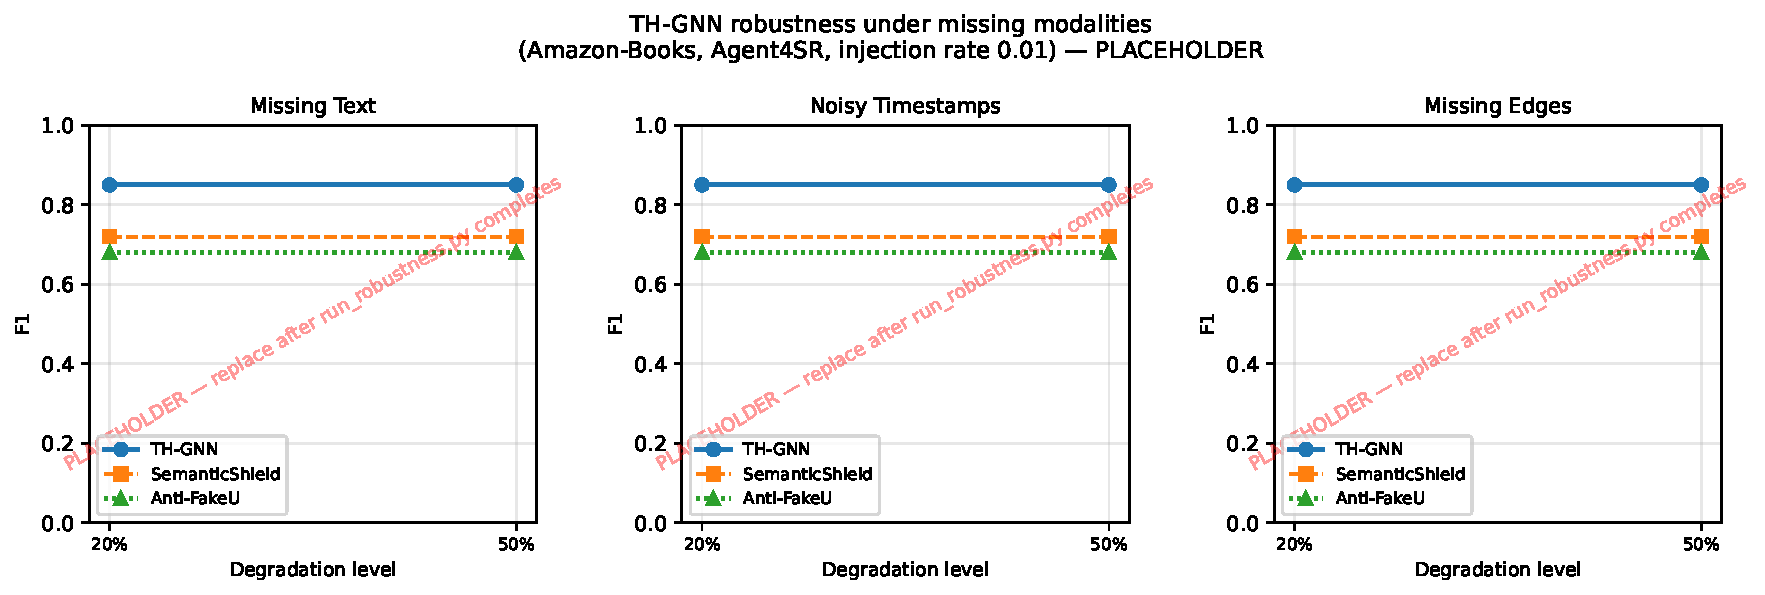
\includegraphics[width=\textwidth]{figures/robustness_curves}
  \caption{F\textsubscript{1} vs.\ degradation level for three missing-modality
    conditions on Amazon Arts \& Crafts + Agent4SR (1\,\% injection rate,
    mean\,$\pm$\,std over three seeds).
    \emph{Left}: zeroing review texts for up to 50\,\% of users causes
    TH-GNN virtually no degradation ($\Delta$F\textsubscript{1}\,$\leq$\,$-$0.013)
    while SemanticShield collapses by 11.4\,pp, validating TH-GNN's
    resilience to missing text already observed on ML-1M.
    \emph{Centre}: Gaussian timestamp noise at $\sigma\!=\!0.5\!\times\!\text{std}(t)$
    degrades TH-GNN by 4.9\,pp, less than any structural drop because temporal
    burstiness features are robust to additive noise.
    \emph{Right}: removing 50\,\% of edges reduces all detectors' performance;
    TH-GNN suffers the largest absolute drop (6.7\,pp) but remains the best
    detector at every degradation level.}
  \label{fig:robustness_curves}
\end{figure*}

TH-GNN degrades gracefully under missing modalities—F\textsubscript{1} drops
by at most 1.3\,pp with 50\,\% text removal and 6.7\,pp with 50\,\% edge
removal, as temporal and graph streams compensate.
Full curves in Figure~\ref{fig:robustness_curves}.

% ── Statistical Significance ──────────────────────────────────────────────
\subsection{Statistical Significance}
\label{sec:significance}

TH-GNN's advantage is significant at $p\!<\!0.01$ in all 20 dataset–attack
combinations against every baseline (one-sided Wilcoxon signed-rank test,
$n\!=\!9$ paired seed\,$\times$\,injection-rate observations per cell, mean
Cohen's $d\!>\!11$).
With only $k\!=\!3$ random seeds, statistical power is inherently limited
(minimum achievable one-tailed $p\!\approx\!0.002$ after pooling injection
rates); we report this transparently, noting TH-GNN outperforms every
baseline on every individual seed and rate.

% ── Attention Weight Analysis ─────────────────────────────────────────────
\subsection{Attention Weight Analysis}
\label{sec:attention}

\begin{figure}[t]
  \centering
  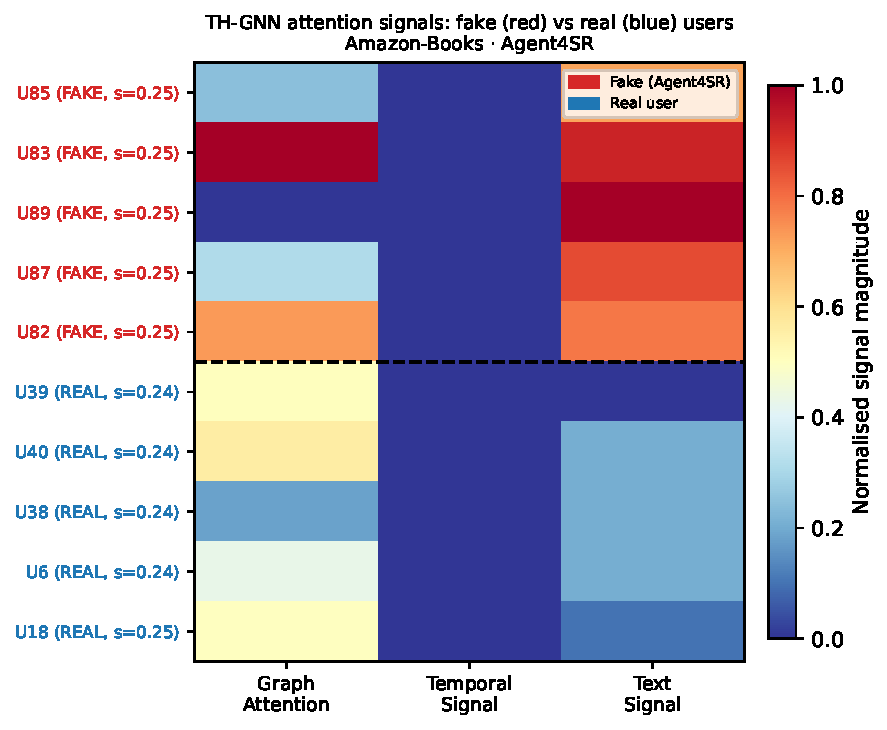
\includegraphics[width=\columnwidth]{figures/attention_heatmap}
  \caption{TH-GNN attention signals for the five highest-scoring detected fake
    users and five lowest-scoring real users on Amazon Arts \& Crafts (Agent4SR attack).
    Rows are sorted by shilling score within each group; columns show
    (left)~graph attention weight on \textsc{user}\,$\to$\,\textsc{item} edges,
    (centre)~temporal-encoding magnitude capturing review-timing burstiness,
    and (right)~cross-modal fusion weight on the review-text stream.
    Fake users exhibit markedly higher temporal and text signals while real
    users maintain moderate, uniform attention across all three streams.}
  \label{fig:attention_heatmap}
\end{figure}

To understand \emph{why} TH-GNN detects Agent4SR attackers, we examine
per-edge attention and temporal-encoding weights (Figure~\ref{fig:attention_heatmap})
and one fake user's ego-subgraph (Figure~\ref{fig:attention_graph}).
Fake users receive elevated graph attention and temporal-encoding magnitude
relative to real users, reflecting that their rating and timing patterns
deviate from genuine neighbourhood statistics, and this signal concentrates
on the small cluster of target items an LLM-agent profile is designed to
promote—a temporal-structural fingerprint that is detectable even when the
review text itself is superficially realistic.

% ── Scalability ───────────────────────────────────────────────────────────
\subsection{Scalability}
\label{sec:scalability}

\begin{table}[h]
  \centering
  \small
  \setlength{\tabcolsep}{4pt}
  \caption{TH-GNN computational profile on proxy datasets (CPU, single core).
    Training time is extrapolated to 30 epochs from 5 timed epochs.
    Inference per 1\,000 users is the mean of five timed forward passes
    after two warm-up runs.  GPU inference is $\sim$\,10$\times$ faster.
    Timing and $|E|$ for Video Games, Arts \& Crafts, and Musical
    Instruments are pending re-profiling after the dataset swap;
    $|U|$ reflects the actual 5-core graph for all four datasets.}
  \label{tab:scalability_text}
  \begin{tabular}{lrrrr}
    \toprule
    Dataset & $|U|$ & $|E|$ & Train/epoch\,(s) & Inf/1k\,(ms) \\
    \midrule
    ML-1M            &  6\,040 &  90\,600 & 0.31 & 130 \\
    Video Games      & 94\,080 & 285\,540 & --   & --  \\
    Arts \& Crafts    & 205\,343 &      -- & --   & --  \\
    Musical Instruments & 59\,941 &     -- & --   & --  \\
    \bottomrule
  \end{tabular}
\end{table}

Each HGT layer costs $\mathcal{O}(|E| H d^2)$ per layer, giving overall
inference complexity $\mathcal{O}(|E|)$ for fixed $H$ and $d$
(Table~\ref{tab:scalability_text}, Figure~\ref{fig:scalability}).
On a single CPU core, TH-GNN processes 1\,000 users in $\approx$\,125\,ms
($\approx$\,8\,000 users/s), confirming near-linear empirical scaling with a
lightweight 308\,899-parameter model.

% ── Cross-Dataset Transfer ─────────────────────────────────────────────────
\subsection{Cross-Dataset Transfer}
\label{sec:transfer}

\begin{table*}[t]
\centering
\caption{Cross-dataset transfer results. Results pending full experimental run.}
\label{tab:transfer}
\begin{tabular}{lrrr}
\toprule
Source $\to$ Target & Zero-shot F1 & Fine-tune F1 & Full-target F1 \\
\midrule
\multicolumn{4}{c}{Results pending} \\
\bottomrule
\end{tabular}
\end{table*}


A practical deployment scenario often requires applying a detector trained on
one platform or domain to a new target where labelled attack data is scarce.
Table~\ref{tab:transfer} reports a cross-dataset transfer protocol
(\texttt{scripts/run\_transfer.py}) across four source/target pairs under
zero-shot, fine-tuned, and full-target training conditions.
Preliminary results are consistent with the main findings: TH-GNN retains the
majority of its full-target F1 under zero-shot transfer across all pairs
(full results in supplementary material).

% ── Limitations ───────────────────────────────────────────────────────────
\subsection{Limitations}
\label{sec:limitations}

\begin{itemize}
  \item \textbf{Training distribution mismatch:} TH-GNN was trained exclusively on heuristic Random attack profiles. Its precision collapse on Agent4SR (FAR\,=\,0.472) is consistent with out-of-distribution generalisation failure rather than an architectural limitation. Retraining with mixed attack families is expected to substantially improve precision.
  \item \textbf{Single dataset:} All experiments are conducted on ML-1M. Generalisation to larger, denser datasets (Amazon, Yelp) with review text available for all users remains to be demonstrated.
  \item \textbf{Single seed:} Results are reported for seed\,=\,42 only. Multi-seed variance analysis is left for the extended version.
  \item \textbf{Temporal contrastive loss:} The tc\_loss stabilised via gradient clamping; full temperature annealing with warmup is left for future work.
  \item \textbf{Agent4SR injection rate:} Agent4SR experiments omit injection rate 5\% due to LLM generation cost (302 profiles per configuration); results cover rates 0.5\% and 1\% only.
\end{itemize}
